% Options for packages loaded elsewhere
\PassOptionsToPackage{unicode}{hyperref}
\PassOptionsToPackage{hyphens}{url}
%
\documentclass[
]{book}
\usepackage{lmodern}
\usepackage{amsmath}
\usepackage{ifxetex,ifluatex}
\ifnum 0\ifxetex 1\fi\ifluatex 1\fi=0 % if pdftex
  \usepackage[T1]{fontenc}
  \usepackage[utf8]{inputenc}
  \usepackage{textcomp} % provide euro and other symbols
  \usepackage{amssymb}
\else % if luatex or xetex
  \usepackage{unicode-math}
  \defaultfontfeatures{Scale=MatchLowercase}
  \defaultfontfeatures[\rmfamily]{Ligatures=TeX,Scale=1}
\fi
% Use upquote if available, for straight quotes in verbatim environments
\IfFileExists{upquote.sty}{\usepackage{upquote}}{}
\IfFileExists{microtype.sty}{% use microtype if available
  \usepackage[]{microtype}
  \UseMicrotypeSet[protrusion]{basicmath} % disable protrusion for tt fonts
}{}
\makeatletter
\@ifundefined{KOMAClassName}{% if non-KOMA class
  \IfFileExists{parskip.sty}{%
    \usepackage{parskip}
  }{% else
    \setlength{\parindent}{0pt}
    \setlength{\parskip}{6pt plus 2pt minus 1pt}}
}{% if KOMA class
  \KOMAoptions{parskip=half}}
\makeatother
\usepackage{xcolor}
\IfFileExists{xurl.sty}{\usepackage{xurl}}{} % add URL line breaks if available
\IfFileExists{bookmark.sty}{\usepackage{bookmark}}{\usepackage{hyperref}}
\hypersetup{
  pdftitle={Empirical Research (with R)},
  pdfauthor={Marco Kühne},
  hidelinks,
  pdfcreator={LaTeX via pandoc}}
\urlstyle{same} % disable monospaced font for URLs
\usepackage{color}
\usepackage{fancyvrb}
\newcommand{\VerbBar}{|}
\newcommand{\VERB}{\Verb[commandchars=\\\{\}]}
\DefineVerbatimEnvironment{Highlighting}{Verbatim}{commandchars=\\\{\}}
% Add ',fontsize=\small' for more characters per line
\usepackage{framed}
\definecolor{shadecolor}{RGB}{248,248,248}
\newenvironment{Shaded}{\begin{snugshade}}{\end{snugshade}}
\newcommand{\AlertTok}[1]{\textcolor[rgb]{0.94,0.16,0.16}{#1}}
\newcommand{\AnnotationTok}[1]{\textcolor[rgb]{0.56,0.35,0.01}{\textbf{\textit{#1}}}}
\newcommand{\AttributeTok}[1]{\textcolor[rgb]{0.77,0.63,0.00}{#1}}
\newcommand{\BaseNTok}[1]{\textcolor[rgb]{0.00,0.00,0.81}{#1}}
\newcommand{\BuiltInTok}[1]{#1}
\newcommand{\CharTok}[1]{\textcolor[rgb]{0.31,0.60,0.02}{#1}}
\newcommand{\CommentTok}[1]{\textcolor[rgb]{0.56,0.35,0.01}{\textit{#1}}}
\newcommand{\CommentVarTok}[1]{\textcolor[rgb]{0.56,0.35,0.01}{\textbf{\textit{#1}}}}
\newcommand{\ConstantTok}[1]{\textcolor[rgb]{0.00,0.00,0.00}{#1}}
\newcommand{\ControlFlowTok}[1]{\textcolor[rgb]{0.13,0.29,0.53}{\textbf{#1}}}
\newcommand{\DataTypeTok}[1]{\textcolor[rgb]{0.13,0.29,0.53}{#1}}
\newcommand{\DecValTok}[1]{\textcolor[rgb]{0.00,0.00,0.81}{#1}}
\newcommand{\DocumentationTok}[1]{\textcolor[rgb]{0.56,0.35,0.01}{\textbf{\textit{#1}}}}
\newcommand{\ErrorTok}[1]{\textcolor[rgb]{0.64,0.00,0.00}{\textbf{#1}}}
\newcommand{\ExtensionTok}[1]{#1}
\newcommand{\FloatTok}[1]{\textcolor[rgb]{0.00,0.00,0.81}{#1}}
\newcommand{\FunctionTok}[1]{\textcolor[rgb]{0.00,0.00,0.00}{#1}}
\newcommand{\ImportTok}[1]{#1}
\newcommand{\InformationTok}[1]{\textcolor[rgb]{0.56,0.35,0.01}{\textbf{\textit{#1}}}}
\newcommand{\KeywordTok}[1]{\textcolor[rgb]{0.13,0.29,0.53}{\textbf{#1}}}
\newcommand{\NormalTok}[1]{#1}
\newcommand{\OperatorTok}[1]{\textcolor[rgb]{0.81,0.36,0.00}{\textbf{#1}}}
\newcommand{\OtherTok}[1]{\textcolor[rgb]{0.56,0.35,0.01}{#1}}
\newcommand{\PreprocessorTok}[1]{\textcolor[rgb]{0.56,0.35,0.01}{\textit{#1}}}
\newcommand{\RegionMarkerTok}[1]{#1}
\newcommand{\SpecialCharTok}[1]{\textcolor[rgb]{0.00,0.00,0.00}{#1}}
\newcommand{\SpecialStringTok}[1]{\textcolor[rgb]{0.31,0.60,0.02}{#1}}
\newcommand{\StringTok}[1]{\textcolor[rgb]{0.31,0.60,0.02}{#1}}
\newcommand{\VariableTok}[1]{\textcolor[rgb]{0.00,0.00,0.00}{#1}}
\newcommand{\VerbatimStringTok}[1]{\textcolor[rgb]{0.31,0.60,0.02}{#1}}
\newcommand{\WarningTok}[1]{\textcolor[rgb]{0.56,0.35,0.01}{\textbf{\textit{#1}}}}
\usepackage{longtable,booktabs}
\usepackage{calc} % for calculating minipage widths
% Correct order of tables after \paragraph or \subparagraph
\usepackage{etoolbox}
\makeatletter
\patchcmd\longtable{\par}{\if@noskipsec\mbox{}\fi\par}{}{}
\makeatother
% Allow footnotes in longtable head/foot
\IfFileExists{footnotehyper.sty}{\usepackage{footnotehyper}}{\usepackage{footnote}}
\makesavenoteenv{longtable}
\usepackage{graphicx}
\makeatletter
\def\maxwidth{\ifdim\Gin@nat@width>\linewidth\linewidth\else\Gin@nat@width\fi}
\def\maxheight{\ifdim\Gin@nat@height>\textheight\textheight\else\Gin@nat@height\fi}
\makeatother
% Scale images if necessary, so that they will not overflow the page
% margins by default, and it is still possible to overwrite the defaults
% using explicit options in \includegraphics[width, height, ...]{}
\setkeys{Gin}{width=\maxwidth,height=\maxheight,keepaspectratio}
% Set default figure placement to htbp
\makeatletter
\def\fps@figure{htbp}
\makeatother
\setlength{\emergencystretch}{3em} % prevent overfull lines
\providecommand{\tightlist}{%
  \setlength{\itemsep}{0pt}\setlength{\parskip}{0pt}}
\setcounter{secnumdepth}{5}
\usepackage{booktabs}
\ifluatex
  \usepackage{selnolig}  % disable illegal ligatures
\fi
\usepackage[]{natbib}
\bibliographystyle{apalike}

\title{Empirical Research (with R)}
\usepackage{etoolbox}
\makeatletter
\providecommand{\subtitle}[1]{% add subtitle to \maketitle
  \apptocmd{\@title}{\par {\large #1 \par}}{}{}
}
\makeatother
\subtitle{Based On True Stories}
\author{Marco Kühne}
\date{2021-08-09}

\begin{document}
\maketitle

{
\setcounter{tocdepth}{1}
\tableofcontents
}
\hypertarget{dust-and-dark}{%
\chapter*{Dust and Dark}\label{dust-and-dark}}
\addcontentsline{toc}{chapter}{Dust and Dark}

A dusty lecture hall. The light cut through the darkness from the left side of the room. A dozen of seats in each bench, only few occupied by small groups of students who were trying to make sure that they sit far from each other and as far as possible from the lecturer. The bearish but competent assistant professor explained how to analyze and evaluate the results of various memory and cognition experiments through boxplots, t-test and the like in that software. My creaky, slow but loyal laptop in front of me. That's where R was introduced in my psychology undergraduate studies.

\hypertarget{introduction}{%
\chapter{Introduction}\label{introduction}}

Hello World

Second hi

\url{https://medium.com/@delucmat/how-to-publish-bookdown-projects-with-github-actions-on-github-pages-6e6aecc7331e}

I need a \_book directory:

The .html files (which were compiled from the .Rmd files) are all stored within the \_book directory which basically serves as a static website.

\hypertarget{literature}{%
\chapter{Literature}\label{literature}}

Here is a review of existing methods.

\url{https://mhweber.github.io/2020/02/12/trying-out-bookdown-and-publishing-to-github-pages/}

\hypertarget{methods}{%
\chapter{Methods}\label{methods}}

We describe our methods in this chapter.

\hypertarget{slope-fields}{%
\chapter{Slope Fields}\label{slope-fields}}

\hypertarget{definition}{%
\section{Definition}\label{definition}}

\begin{quote}
Slope fields (also called direction fields) are a graphical representation of the solutions to a first-order differential equation of a scalar function. Solutions to a slope field are functions drawn as solid curves. A slope field shows the slope of a differential equation at certain vertical and horizontal intervals on the x-y plane, and can be used to determine the approximate tangent slope at a point on a curve, where the curve is some solution to the differential equation.

\hfill Wikipedia contributors. (2021, May 17). Slope field. In Wikipedia, The Free Encyclopedia. Retrieved 05:51, June 16, 2021, from \url{https://en.wikipedia.org/w/index.php?title=Slope_field\&oldid=1023635282}
\end{quote}

\hypertarget{slope-fields-in-r}{%
\section{Slope Fields in R}\label{slope-fields-in-r}}

There's no need to build everything from scratch. The first useful resource I can find is:

\url{https://www.r-bloggers.com/2014/09/generate-slope-fields-in-r-and-python/}

Show me the code.

\begin{Shaded}
\begin{Highlighting}[]
\CommentTok{\# Our differential equation}
\NormalTok{diff }\OtherTok{\textless{}{-}} \ControlFlowTok{function}\NormalTok{(x,y)}
\NormalTok{\{}
  \FunctionTok{return}\NormalTok{(x}\SpecialCharTok{/}\NormalTok{y) }\CommentTok{\#Try also x+y}
\NormalTok{\}}

\CommentTok{\# Line function}
\NormalTok{TheLine }\OtherTok{\textless{}{-}} \ControlFlowTok{function}\NormalTok{(x1,y1,slp,d)}
\NormalTok{\{}
\NormalTok{  z }\OtherTok{=}\NormalTok{ slope}\SpecialCharTok{*}\NormalTok{(d}\SpecialCharTok{{-}}\NormalTok{x1)}\SpecialCharTok{+}\NormalTok{y1}
  \FunctionTok{return}\NormalTok{(z)}
\NormalTok{\}}

\CommentTok{\# Domains}
\NormalTok{x }\OtherTok{=} \FunctionTok{seq}\NormalTok{(}\SpecialCharTok{{-}}\DecValTok{20}\NormalTok{,}\DecValTok{20}\NormalTok{,}\FloatTok{0.5}\NormalTok{)}
\NormalTok{y }\OtherTok{=} \FunctionTok{seq}\NormalTok{(}\SpecialCharTok{{-}}\DecValTok{20}\NormalTok{,}\DecValTok{20}\NormalTok{,}\FloatTok{0.5}\NormalTok{)}

\CommentTok{\# Points to draw our graph}
\NormalTok{f }\OtherTok{=} \FunctionTok{c}\NormalTok{(}\SpecialCharTok{{-}}\DecValTok{5}\NormalTok{,}\DecValTok{5}\NormalTok{) }
\NormalTok{h }\OtherTok{=} \FunctionTok{c}\NormalTok{(}\SpecialCharTok{{-}}\DecValTok{5}\NormalTok{,}\DecValTok{5}\NormalTok{)}
\FunctionTok{plot}\NormalTok{(f,h,}\AttributeTok{main=}\StringTok{"Slope field"}\NormalTok{)}


\CommentTok{\# Let\textquotesingle{}s generate the slope field}
\ControlFlowTok{for}\NormalTok{(j }\ControlFlowTok{in}\NormalTok{ x)}
\NormalTok{\{}
  \ControlFlowTok{for}\NormalTok{(k }\ControlFlowTok{in}\NormalTok{ y)}
\NormalTok{  \{}
\NormalTok{    slope }\OtherTok{=} \FunctionTok{diff}\NormalTok{(j,k)}
\NormalTok{    domain }\OtherTok{=} \FunctionTok{seq}\NormalTok{(j}\FloatTok{{-}0.07}\NormalTok{,j}\FloatTok{+0.07}\NormalTok{,}\FloatTok{0.14}\NormalTok{)}
\NormalTok{    z }\OtherTok{=} \FunctionTok{TheLine}\NormalTok{(j,k,slope,domain)}
    \FunctionTok{arrows}\NormalTok{(domain[}\DecValTok{1}\NormalTok{],z[}\DecValTok{1}\NormalTok{],domain[}\DecValTok{2}\NormalTok{],z[}\DecValTok{2}\NormalTok{],}\AttributeTok{length=}\FloatTok{0.08}\NormalTok{)}
\NormalTok{  \}}
\NormalTok{\}}
\end{Highlighting}
\end{Shaded}

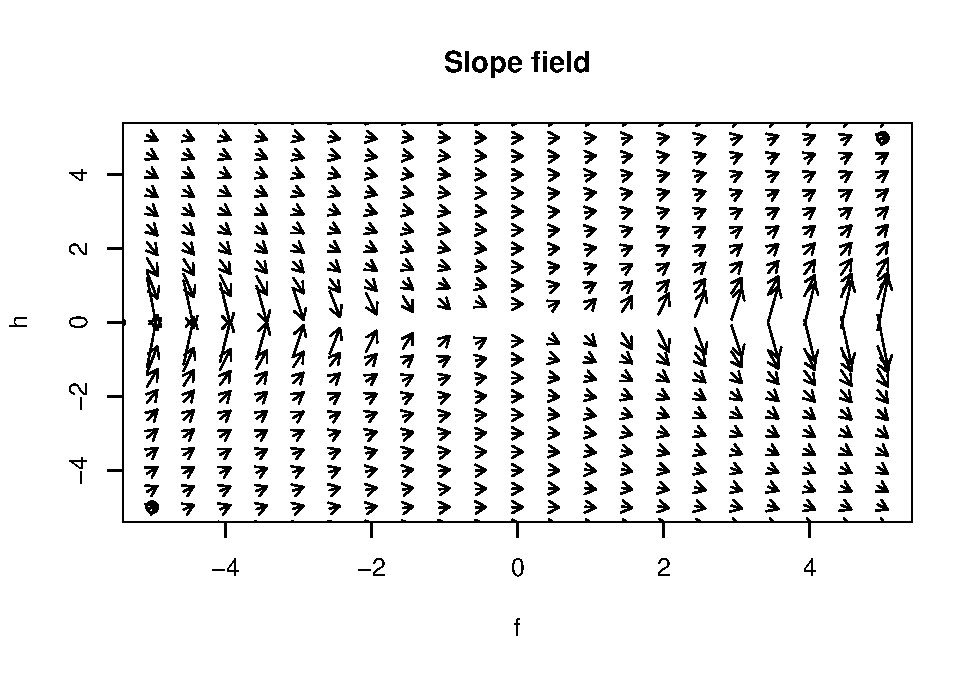
\includegraphics{Empirical-Research_files/figure-latex/unnamed-chunk-1-1.pdf}

The post \url{https://stackoverflow.com/questions/47984874/how-to-create-a-slope-field-in-r} puts this into a \texttt{SlopeField} function.

Show me the code.

\begin{Shaded}
\begin{Highlighting}[]
\NormalTok{SlopeField }\OtherTok{=} \ControlFlowTok{function}\NormalTok{(FUN,}\AttributeTok{xi =} \SpecialCharTok{{-}}\DecValTok{5}\NormalTok{,}\AttributeTok{xs =} \DecValTok{5}\NormalTok{,}\AttributeTok{yi =} \SpecialCharTok{{-}}\DecValTok{5}\NormalTok{,}\AttributeTok{ys =} \DecValTok{5}\NormalTok{, }\AttributeTok{radius =} \FloatTok{0.1}\NormalTok{, }\AttributeTok{grid.by =} \FloatTok{0.25}\NormalTok{)\{}
  \CommentTok{\# FUN   {-} given function ODE i.e:  }
  \CommentTok{\# xi,xs {-} lower and upper bound {-} x {-} plot}
  \CommentTok{\# yi,ys {-} lower and upper bound {-} y {-} plot}
  
  \CommentTok{\# grid points}
\NormalTok{  seqx }\OtherTok{=} \FunctionTok{seq}\NormalTok{(xi,xs,grid.by)}
\NormalTok{  seqy }\OtherTok{=} \FunctionTok{seq}\NormalTok{(yi,ys,grid.by)}
  
  \CommentTok{\# plot}
\NormalTok{  f }\OtherTok{=} \FunctionTok{c}\NormalTok{(xi,xs) }
\NormalTok{  h }\OtherTok{=} \FunctionTok{c}\NormalTok{(yi,ys)}
  \FunctionTok{plot}\NormalTok{(f,h,}\AttributeTok{main=}\StringTok{"Slope field"}\NormalTok{, }\AttributeTok{ylab =} \StringTok{"Dependet variable"}\NormalTok{, }\AttributeTok{xlab =} \StringTok{"Independet variable"}\NormalTok{, }\AttributeTok{pch =} \StringTok{"."}\NormalTok{)}
  
  \CommentTok{\# arrows}
  
  \ControlFlowTok{for}\NormalTok{(x }\ControlFlowTok{in}\NormalTok{ seqx)\{}
    \ControlFlowTok{for}\NormalTok{(y }\ControlFlowTok{in}\NormalTok{ seqy)\{}
\NormalTok{      ym }\OtherTok{=}\NormalTok{ y}
\NormalTok{      xm }\OtherTok{=}\NormalTok{ x}
      
\NormalTok{      slope }\OtherTok{=} \FunctionTok{unlist}\NormalTok{(}\FunctionTok{FUN}\NormalTok{(x,y))}
      
      \ControlFlowTok{if}\NormalTok{(}\FunctionTok{is.na}\NormalTok{(slope))\{}
\NormalTok{        cor }\OtherTok{=} \StringTok{"black"}
\NormalTok{      \} }\ControlFlowTok{else} \ControlFlowTok{if}\NormalTok{(slope }\SpecialCharTok{\textgreater{}} \DecValTok{0}\NormalTok{)\{}
\NormalTok{        cor }\OtherTok{=} \StringTok{"blue"}
\NormalTok{      \}}\ControlFlowTok{else} \ControlFlowTok{if}\NormalTok{ (slope }\SpecialCharTok{\textless{}} \DecValTok{0}\NormalTok{) \{}
\NormalTok{        cor }\OtherTok{=} \StringTok{"red"}
\NormalTok{      \}}\ControlFlowTok{else} \ControlFlowTok{if}\NormalTok{(slope }\SpecialCharTok{==} \DecValTok{0}\NormalTok{) \{}
\NormalTok{        cor }\OtherTok{=} \StringTok{"green"}
\NormalTok{      \}}
      \FunctionTok{arrows}\NormalTok{(radius}\SpecialCharTok{*}\FunctionTok{cos}\NormalTok{(}\FunctionTok{atan}\NormalTok{(slope)}\SpecialCharTok{+}\NormalTok{pi)}\SpecialCharTok{+}\NormalTok{xm,}
\NormalTok{             radius}\SpecialCharTok{*}\FunctionTok{sin}\NormalTok{(}\FunctionTok{atan}\NormalTok{(slope)}\SpecialCharTok{+}\NormalTok{pi)}\SpecialCharTok{+}\NormalTok{ym,}
\NormalTok{             radius}\SpecialCharTok{*}\FunctionTok{cos}\NormalTok{(}\FunctionTok{atan}\NormalTok{(slope))}\SpecialCharTok{+}\NormalTok{xm,}
\NormalTok{             radius}\SpecialCharTok{*}\FunctionTok{sin}\NormalTok{(}\FunctionTok{atan}\NormalTok{(slope))}\SpecialCharTok{+}\NormalTok{ym, }
             \AttributeTok{length =} \FloatTok{0.2}\SpecialCharTok{*}\NormalTok{radius, }\AttributeTok{col=}\NormalTok{ cor)}
\NormalTok{    \}}
\NormalTok{  \}}
\NormalTok{\}}
\end{Highlighting}
\end{Shaded}

\hypertarget{technical-example}{%
\section{Technical Example}\label{technical-example}}

We can specify an ODE in another function and plot its slope field. The suggested example is

\[y'(t) = y^2 - t \]

\begin{Shaded}
\begin{Highlighting}[]
\NormalTok{ode }\OtherTok{=} \ControlFlowTok{function}\NormalTok{(t, y)\{}
\NormalTok{  dydt }\OtherTok{\textless{}{-}}\NormalTok{ y}\SpecialCharTok{\^{}}\DecValTok{2}\SpecialCharTok{{-}}\NormalTok{t}
  \FunctionTok{list}\NormalTok{(dydt)}
\NormalTok{\}}
\end{Highlighting}
\end{Shaded}

Let's draw the slope field.

\begin{Shaded}
\begin{Highlighting}[]
\FunctionTok{SlopeField}\NormalTok{(ode, }\AttributeTok{xi =} \SpecialCharTok{{-}}\DecValTok{2}\NormalTok{, }\AttributeTok{xs =} \DecValTok{5}\NormalTok{, }\AttributeTok{yi =} \SpecialCharTok{{-}}\DecValTok{2}\NormalTok{, }\AttributeTok{ys =} \DecValTok{2}\NormalTok{,}\AttributeTok{radius =} \FloatTok{0.1}\NormalTok{, }\AttributeTok{grid.by =} \FloatTok{0.25}\NormalTok{)}
\end{Highlighting}
\end{Shaded}

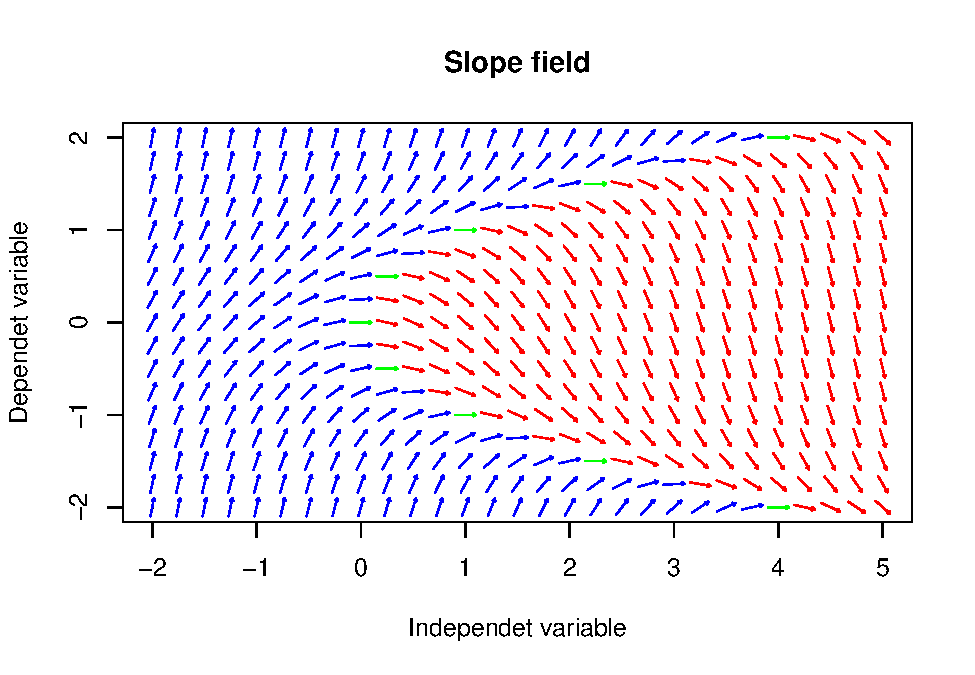
\includegraphics{Empirical-Research_files/figure-latex/unnamed-chunk-4-1.pdf}

That looks good. But can how can we get the ODE solution from this graph?

\hypertarget{understandable-examples}{%
\section{Understandable Examples}\label{understandable-examples}}

\hypertarget{y-y}{%
\subsection{y' = y}\label{y-y}}

Even without a background in differential equations, think about the following:

\[y'(x) = y(x)\]
We are looking for a function \(y(x)\) that is identical to its first derivative \(y'(x)\). Perhaps you remember such a function from your last math class (analysis). It is the exponential function, that basically does not change by differentiation.

\[y(x) = e^x \Rightarrow y'(x) = e^x \]

\begin{Shaded}
\begin{Highlighting}[]
\NormalTok{ode\_1 }\OtherTok{=} \ControlFlowTok{function}\NormalTok{(t, y)\{}
\NormalTok{  dydt }\OtherTok{\textless{}{-}}\NormalTok{ y}
  \FunctionTok{list}\NormalTok{(dydt)}
\NormalTok{\}}

\FunctionTok{SlopeField}\NormalTok{(ode\_1, }\AttributeTok{xi =} \SpecialCharTok{{-}}\DecValTok{2}\NormalTok{, }\AttributeTok{xs =} \DecValTok{5}\NormalTok{, }\AttributeTok{yi =} \SpecialCharTok{{-}}\DecValTok{2}\NormalTok{, }\AttributeTok{ys =} \DecValTok{2}\NormalTok{,}\AttributeTok{radius =} \FloatTok{0.1}\NormalTok{, }\AttributeTok{grid.by =} \FloatTok{0.25}\NormalTok{)}
\end{Highlighting}
\end{Shaded}

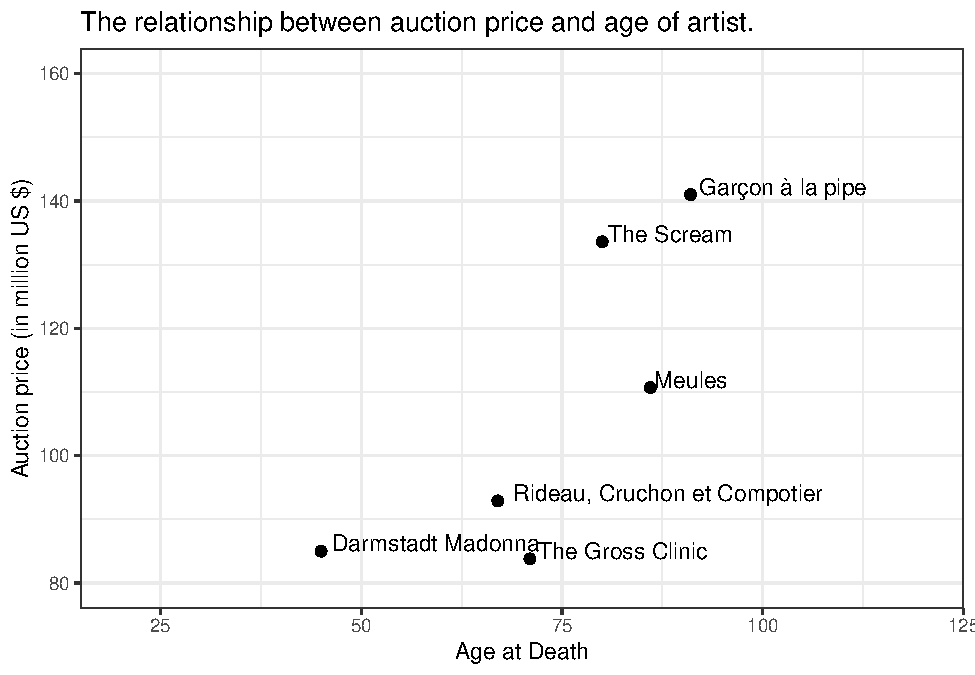
\includegraphics{Empirical-Research_files/figure-latex/unnamed-chunk-5-1.pdf}

Can you see something like the exponential function in this slope field?

Show me how an exponential function looks like.

\begin{Shaded}
\begin{Highlighting}[]
\NormalTok{x\_value}\OtherTok{\textless{}{-}}\FunctionTok{runif}\NormalTok{(}\DecValTok{100}\NormalTok{,}\DecValTok{2}\NormalTok{,}\DecValTok{8}\NormalTok{)}
\FunctionTok{plot}\NormalTok{(x\_value,}\FunctionTok{exp}\NormalTok{(x\_value))}
\end{Highlighting}
\end{Shaded}

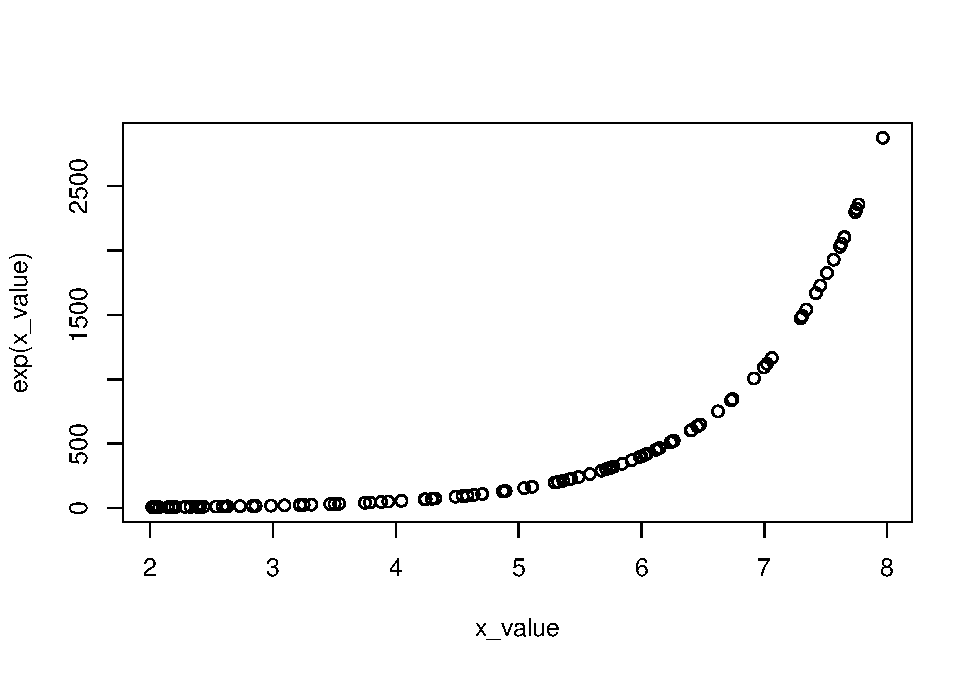
\includegraphics{Empirical-Research_files/figure-latex/unnamed-chunk-6-1.pdf}

Perhaps you can spot something like the \(y(x) = e^x\) in the blue area. But how about the red arrows? Any mirror at the x-axis is also a valid solution to the problem. How do we mirror? Use a factor in front of the e function. This may be negative.

\[y(x) = C \cdot e^x \Rightarrow y'(x) = C \cdot e^x \]

\hypertarget{y--y}{%
\subsection{y' = -y}\label{y--y}}

Let's give it another try. Which function equals its first derivative (after changing sign).

\[y'(x) = -y(x)\]

It is a sibling of the \(e^x\). The solution is \(y(x) = C \cdot e^{-x}\).

\begin{Shaded}
\begin{Highlighting}[]
\NormalTok{ode\_2 }\OtherTok{=} \ControlFlowTok{function}\NormalTok{(t, y)\{}
\NormalTok{  dydt }\OtherTok{\textless{}{-}} \SpecialCharTok{{-}}\NormalTok{y}
  \FunctionTok{list}\NormalTok{(dydt)}
\NormalTok{\}}

\FunctionTok{SlopeField}\NormalTok{(ode\_2, }\AttributeTok{xi =} \SpecialCharTok{{-}}\DecValTok{2}\NormalTok{, }\AttributeTok{xs =} \DecValTok{5}\NormalTok{, }\AttributeTok{yi =} \SpecialCharTok{{-}}\DecValTok{2}\NormalTok{, }\AttributeTok{ys =} \DecValTok{2}\NormalTok{,}\AttributeTok{radius =} \FloatTok{0.1}\NormalTok{, }\AttributeTok{grid.by =} \FloatTok{0.25}\NormalTok{)}
\end{Highlighting}
\end{Shaded}

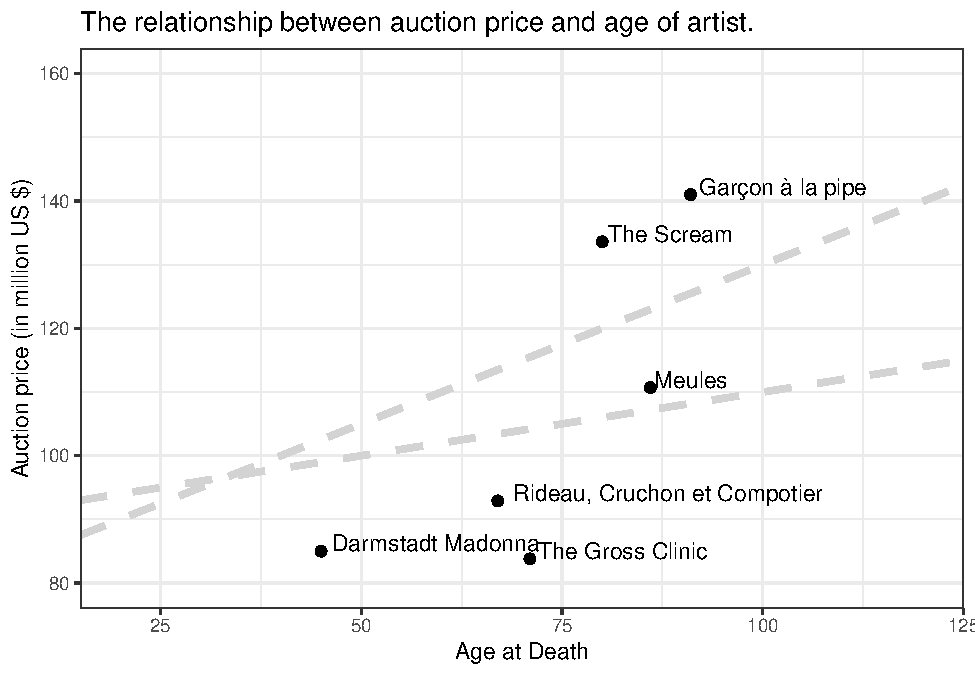
\includegraphics{Empirical-Research_files/figure-latex/unnamed-chunk-7-1.pdf}

\hypertarget{y-x2}{%
\subsection{y' = x\^{}2}\label{y-x2}}

Wait, there's no more y on the RHS. Don't worry. That'll make it even easier. What is the integral of \(x^2\)? You may expect

\[y'(x) = x^2 \Rightarrow \int x^2 dx = 1/3 \cdot x^3 + C\]
Okay, the general shape is a cubic function. Can you spot a cubic function?

\begin{Shaded}
\begin{Highlighting}[]
\NormalTok{ode\_3 }\OtherTok{=} \ControlFlowTok{function}\NormalTok{(t, y)\{}
\NormalTok{  dydt }\OtherTok{\textless{}{-}}\NormalTok{ t}\SpecialCharTok{\^{}}\DecValTok{2}
  \FunctionTok{list}\NormalTok{(dydt)}
\NormalTok{\}}

\FunctionTok{SlopeField}\NormalTok{(ode\_3, }\AttributeTok{xi =} \SpecialCharTok{{-}}\DecValTok{2}\NormalTok{, }\AttributeTok{xs =} \DecValTok{5}\NormalTok{, }\AttributeTok{yi =} \SpecialCharTok{{-}}\DecValTok{2}\NormalTok{, }\AttributeTok{ys =} \DecValTok{2}\NormalTok{,}\AttributeTok{radius =} \FloatTok{0.1}\NormalTok{, }\AttributeTok{grid.by =} \FloatTok{0.25}\NormalTok{)}
\end{Highlighting}
\end{Shaded}

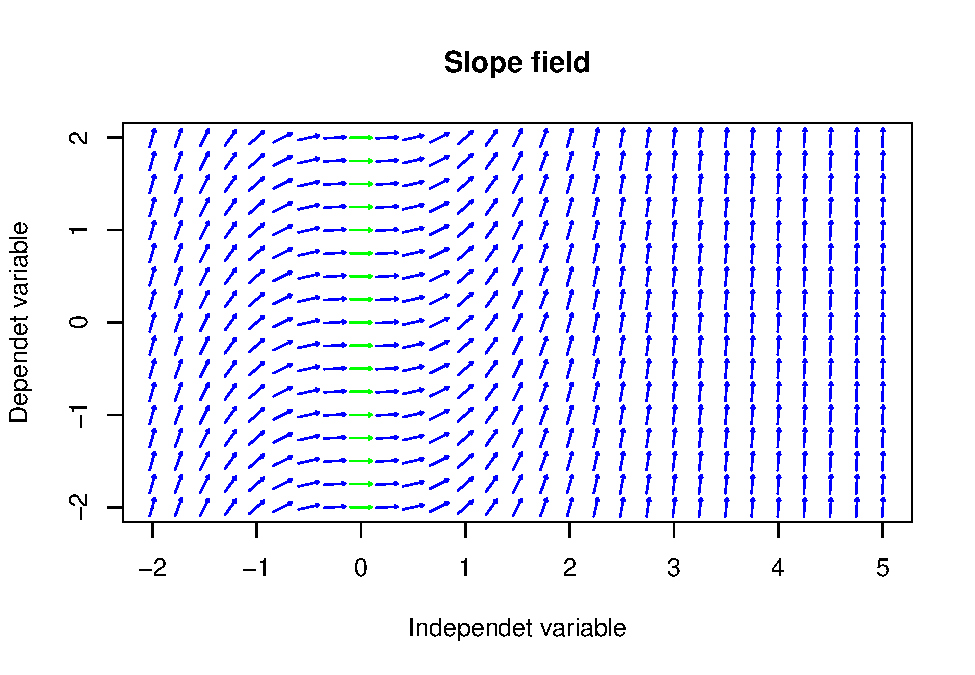
\includegraphics{Empirical-Research_files/figure-latex/unnamed-chunk-8-1.pdf}

\hypertarget{initial-value-problem}{%
\section{Initial value problem}\label{initial-value-problem}}

Recap, the prior solution was \(y(x) = 1/3 \cdot x^3 + C\). Due to \(C\) this is a family of curves. If we specify some of them, that's called the initial value problem. This \emph{problem} makes is actually even more easy to understand the slope field. Let's add two particular cubic functions for \(C = 0\) and \(C = 0.5\).

\begin{Shaded}
\begin{Highlighting}[]
\FunctionTok{SlopeField}\NormalTok{(ode\_3, }\AttributeTok{xi =} \SpecialCharTok{{-}}\DecValTok{2}\NormalTok{, }\AttributeTok{xs =} \DecValTok{5}\NormalTok{, }\AttributeTok{yi =} \SpecialCharTok{{-}}\DecValTok{2}\NormalTok{, }\AttributeTok{ys =} \DecValTok{2}\NormalTok{,}\AttributeTok{radius =} \FloatTok{0.1}\NormalTok{, }\AttributeTok{grid.by =} \FloatTok{0.25}\NormalTok{)}
\FunctionTok{lines}\NormalTok{(y,}\DecValTok{1}\SpecialCharTok{/}\DecValTok{3}\SpecialCharTok{*}\NormalTok{x}\SpecialCharTok{*}\NormalTok{x}\SpecialCharTok{*}\NormalTok{x,}\AttributeTok{col=}\StringTok{"red"}\NormalTok{, }\AttributeTok{lwd=}\DecValTok{2}\NormalTok{)}
\FunctionTok{lines}\NormalTok{(y,}\DecValTok{1}\SpecialCharTok{/}\DecValTok{3}\SpecialCharTok{*}\NormalTok{x}\SpecialCharTok{*}\NormalTok{x}\SpecialCharTok{*}\NormalTok{x}\FloatTok{+0.5}\NormalTok{,}\AttributeTok{col=}\StringTok{"orange"}\NormalTok{, }\AttributeTok{lwd=}\DecValTok{2}\NormalTok{)}
\end{Highlighting}
\end{Shaded}

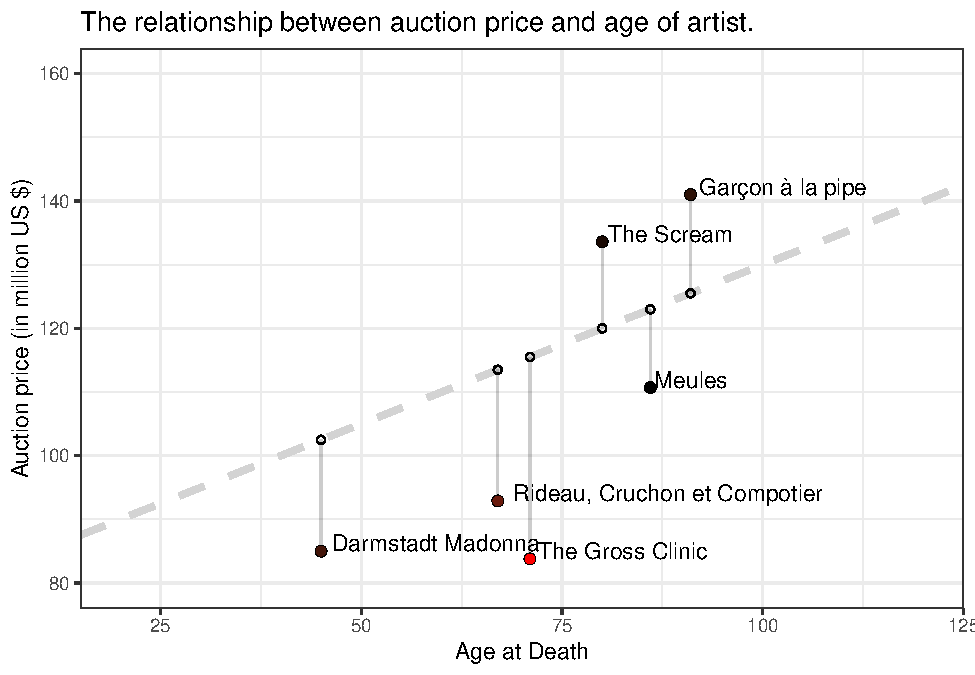
\includegraphics{Empirical-Research_files/figure-latex/unnamed-chunk-9-1.pdf}

Enjoy. Learn. Share.

\hypertarget{git-and-github}{%
\chapter{Git and Github}\label{git-and-github}}

\hypertarget{install-github-and-git}{%
\section{Install Github and Git}\label{install-github-and-git}}

\begin{itemize}
\tightlist
\item
  Get RStudio \url{https://www.rstudio.com/products/rstudio/download/}
\item
  Get Github account \url{https://github.com/}
\item
  Set up Github pages \url{https://pages.github.com/}
\item
  Download Git \url{https://git-scm.com/}
\end{itemize}

Create a ``special repository'' for GitHub Pages. Only this can turn the branch into docs (1 for free).

\begin{itemize}
\tightlist
\item
  Repository: \url{https://github.com/MarcoKuehne/marcokuehne.github.io}
\item
  Homepage: \url{https://marcokuehne.github.io/}
\end{itemize}

Create (or re-open) your R project inside RStudio.

In R console use \texttt{usethis::use\_git()} which always gives three different answers in random order. Confirm accordingly.

\hypertarget{working-with-git}{%
\section{Working with Git}\label{working-with-git}}

Use the terminal inside RStudio. Copy paste into terminal with: \texttt{CTRL\ +\ SHIFT\ +\ V}.

\hypertarget{git-version}{%
\subsection{git version}\label{git-version}}

Let's start with commands that cannot do any harm (it's 2.32 in 08/2021):

\begin{verbatim}
git version
\end{verbatim}

\hypertarget{git-config}{%
\subsection{git config}\label{git-config}}

First, configure github user information on your system. Use the R builtin terminal:

\begin{verbatim}
git config --global user.email MAIL
git config --global user.name NAME
\end{verbatim}

Now, you can commit (upload) changes from RStudio to Github Pages. Check out \texttt{git\ config\ -\/-list}.

\hypertarget{git-init}{%
\subsection{git init}\label{git-init}}

Use \texttt{git\ init} to initialize the repository. It is used to create a new empty repository or directory consisting of files' with the hidden directory. `.git' is created at the top level of your project, which places all of the revision information in one place.

Show what is connected with:

\begin{verbatim}
git remote -v show
\end{verbatim}

\hypertarget{git-status-and-diff}{%
\subsection{git status and diff}\label{git-status-and-diff}}

Shows you which files are in this staging area, and which files have changes that haven't yet been put there. In order to compare the file as it currently is to what you last saved, you can use \texttt{git\ diff\ filename}, e.g.~\texttt{git\ diff\ README.md} in the terminal. \texttt{git\ diff} without any file names will show you all the changes in your repository, while git diff directory will show you the changes to the files in some directory.

\hypertarget{git-commit}{%
\subsection{git commit}\label{git-commit}}

To save the changes in the staging area, you use the command \texttt{git\ commit}. It always saves everything that is in the staging area as one unit: as you will see later, when you want to undo changes to a project, you undo all of a commit or none of it.

Commit requires a message (comment). How to write a good git commit \url{message:l}

\url{https://chris.beams.io/posts/git-commit/}

\hypertarget{git-add}{%
\subsection{git add}\label{git-add}}

\ldots{}

\hypertarget{git-remote-add}{%
\subsection{git remote add}\label{git-remote-add}}

I would like to have something like \texttt{git\ remote\ add\ ...} and \texttt{git\ push\ ...}, not working.

I can add and remove origins, don't know what it means: \texttt{git\ remote\ rm\ origin}

Use git add . in your bash to add all the files to the given folder.

Use git status in your bash to view all the files which are going to be staged to the first commit.

Create \textbf{git remote add}

git remote add origin \url{https://github.com/MarcoKuehne/marcokuehne.github.git}
git remote add origin \url{https://github.com/MarcoKuehne/marcokuehne.github.io}
git remote add origin \url{https://github.com/MarcoKuehne/marcokuehne.github.io.git}

git remote add \href{mailto:git@github.com}{\nolinkurl{git@github.com}}:/.git
git remote add \href{mailto:git@github.com}{\nolinkurl{git@github.com}}:MarcoKuehne/marcokuehne.github.git
git remote add \href{mailto:git@github.com}{\nolinkurl{git@github.com}}:MarcoKuehne/marcokuehne.github.io does not appear to be a repository
git remote add \href{mailto:git@github.com}{\nolinkurl{git@github.com}}:MarcoKuehne/marcokuehne.github.io.git combine both

\hypertarget{git-push}{%
\subsection{git push}\label{git-push}}

git push -u origin main
git push -u origin master
git push origin master
git push origin main
git push --set-upstream origin main
git push -f origin main \# worked somehow!!!

If positive, it asks for github credentials.

\url{https://www.datacamp.com/community/tutorials/git-push-pull}

\hypertarget{basic-routines}{%
\section{Basic Routines}\label{basic-routines}}

\hypertarget{add-commit-push}{%
\subsection{Add + Commit + Push}\label{add-commit-push}}

I make changes to any one of my markdown files, e.g.~the \texttt{README.md} (this can also be done via GitHub web interface) on my local machine. After notoriously saving this on my local machine (STRG+S) it appears in the \emph{stage area} in the right upper panel in RStudio. Commit and push can be either done in RStudio or via terminal line (also in RStudio).

First, let's do it via ``clicking''. Select the staged file. Click ``commit''. A new windows opens and displays the changes in your file. Write a new commit message of amend a previous commit. Click ``close''. From this additional window (or the right upper panel in RStudio) click the green push arrow. Hopefully it will say ``HEAD -\textgreater{} main''. Close. Done. The result should be available on your github repository immediately.

The same procedure via the terminal:

\begin{verbatim}
git add 05-git.Rmd
git commit -m "Updated the git short tutorial"
git push 
\end{verbatim}

How to push? Easy \ldots{}

I need to \texttt{pull} these changes into RStudio. Check the right upper panel ``Diff''. Select \texttt{pull}. You can also find big blue down and green up arrows.

I add this sentence. I save on RStudio, thus it appears as a change to \texttt{README.md} in the Git panel. I select this file and green up arrow (push). I enter my credentials and close (see \url{https://docs.github.com/en/get-started/getting-started-with-git/why-is-git-always-asking-for-my-password}). Here you might use a personal access token. I click \texttt{commit}, enter a commit message, click \texttt{commit} again and close the extra window.

\hypertarget{resources}{%
\section{Resources}\label{resources}}

You can start reading about bookdowns from the inventor:

\url{https://bookdown.org/yihui/bookdown/}

This is pretty advanced and I can't understand a tiny piece of it.

Another option is to start a repo and book by copying ``awesome book'' from another repo.

\url{https://jules32.github.io/bookdown-tutorial/setup.html}

This tutorial worked to push a book to a standard repo. But there were problem with the doc branch.

After I forgot how to start my project or where to find it, I checked:

\url{https://happygitwithr.com/rstudio-git-github.html\#make-local-changes-save-commit}

started a new project with my repo link and a new session. This forks or fetches or pulls or downloads the repo. Now I will try to re-upload the minimal change from today.

Another personal description can be found here:

\url{https://rachaellappan.github.io/bookdown/}

\begin{verbatim}
This enourmously helped with the understanding of commits and pushs on git:

<http://www.differencebetween.net/technology/difference-between-commit-and-push/>
\end{verbatim}

\begin{itemize}
\tightlist
\item
  \texttt{git\ commit\ -m\ "Started\ book"}
\end{itemize}

I followed the video ``How to create a bookdown book in 5 minutes'':

\url{https://www.youtube.com/watch?v=m5D-yoH416Y}

It did not work.

Explaining terminology:

\url{https://www.notion.so/zarkom/Introduction-to-Git-ac396a0697704709a12b6a0e545db049}

Learn Git in 15 Min:

\url{https://www.youtube.com/watch?v=USjZcfj8yxE}

Learn GitHub in 20 Min:

\url{https://www.youtube.com/watch?v=nhNq2kIvi9s}

  \bibliography{book.bib,packages.bib}

\end{document}
